\documentclass{article}
% translate with >> pdflatex -shell-escape <file>

% This file is an extract of the PGFPLOTS manual, copyright by Christian Feuersaenger.
% 
% Feel free to use it as long as you cite the pgfplots manual properly.
%
% See
%   http://pgfplots.sourceforge.net/pgfplots.pdf
% for the complete manual.
%
% Any required input files (for <plot table> or <plot file> or the table package) can be downloaded
% at
% http://www.ctan.org/tex-archive/graphics/pgf/contrib/pgfplots/doc/latex/
% and
% http://www.ctan.org/tex-archive/graphics/pgf/contrib/pgfplots/doc/latex/plotdata/

\usepackage{pgfplots}
\pgfplotsset{compat=newest}

\pagestyle{empty}

\begin{document}
\pgfplotsset{
	samples=15,
	width=7cm,
	xlabel=$x$,
	ylabel=$f(x)$,
	extra y ticks={45},
	legend style={at={(0.03,0.97)},
		anchor=north west}}

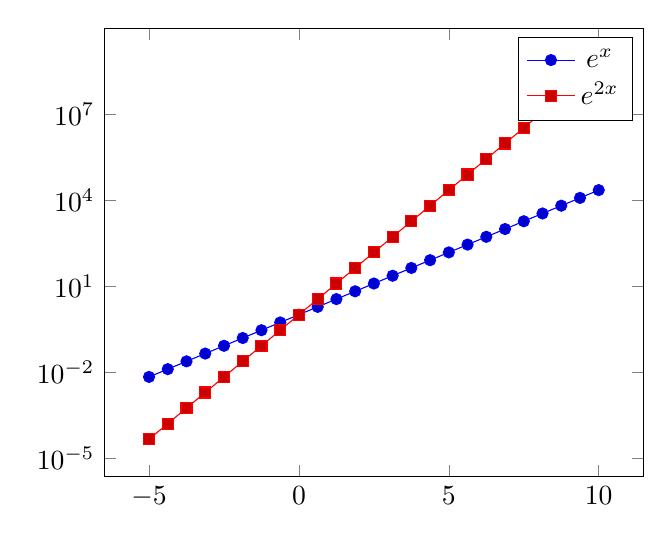
\begin{tikzpicture}
\begin{semilogyaxis}[
	log plot exponent style/.style={
		/pgf/number format/fixed,
		/pgf/number format/use comma,
		/pgf/number format/precision=2},
	domain=-5:10]

	\addplot {exp(x)};
	\addplot {exp(2*x)};

	\legend{$e^x$,$e^{2x}$}
\end{semilogyaxis}
\end{tikzpicture}
\end{document}
